\documentclass[a4paper]{book}
\usepackage{makeidx}
\usepackage{natbib}
\usepackage{graphicx}
\usepackage{multicol}
\usepackage{float}
\usepackage{listings}
\usepackage{color}
\usepackage{ifthen}
\usepackage[table]{xcolor}
\usepackage{textcomp}
\usepackage{alltt}
\usepackage{ifpdf}
\ifpdf
\usepackage[pdftex,
            pagebackref=true,
            colorlinks=true,
            linkcolor=blue,
            unicode
           ]{hyperref}
\else
\usepackage[ps2pdf,
            pagebackref=true,
            colorlinks=true,
            linkcolor=blue,
            unicode
           ]{hyperref}
\usepackage{pspicture}
\fi
\usepackage[utf8]{inputenc}
\usepackage{polski}
\usepackage[T1]{fontenc}

\usepackage{mathptmx}
\usepackage[scaled=.90]{helvet}
\usepackage{courier}
\usepackage{sectsty}
\usepackage[titles]{tocloft}
\usepackage{doxygen}
\lstset{language=C++,inputencoding=utf8,basicstyle=\footnotesize,breaklines=true,breakatwhitespace=true,tabsize=8,numbers=left }
\makeindex
\setcounter{tocdepth}{3}
\renewcommand{\footrulewidth}{0.4pt}
\renewcommand{\familydefault}{\sfdefault}
\hfuzz=15pt
\setlength{\emergencystretch}{15pt}
\hbadness=750
\tolerance=750
\begin{document}
\hypersetup{pageanchor=false,citecolor=blue}
\begin{titlepage}
\vspace*{7cm}
\begin{center}
{\Large \-Sortowania }\\
\vspace*{1cm}
{\large \-Wygenerowano przez Doxygen 1.7.6.1}\\
\vspace*{0.5cm}
{\small Mon May 5 2014 00:34:56}\\
\end{center}
\end{titlepage}
\clearemptydoublepage
\pagenumbering{roman}
\tableofcontents
\clearemptydoublepage
\pagenumbering{arabic}
\hypersetup{pageanchor=true,citecolor=blue}
\chapter{\-Dokumentacja zadania \-P\-A\-M\-S\-I \-L\-A\-B 4}
\label{index}\hypertarget{index}{}\begin{DoxyAuthor}{\-Autor}
\-Martyna \-Bandura 
\end{DoxyAuthor}
\begin{DoxyDate}{\-Data}
19.\-03.\-2014 
\end{DoxyDate}

\chapter{\-Struktura katalogów}
\section{\-Katalogi}
\-Ta struktura katalogów jest posortowana jest z grubsza, choć nie całkowicie, alfabetycznie\-:\begin{DoxyCompactList}
\item \contentsline{section}{prj}{\pageref{dir_9f92f53661fd78c561fa1672d6c740cd}}{}
\end{DoxyCompactList}

\chapter{\-Indeks klas}
\section{\-Lista klas}
\-Tutaj znajdują się klasy, struktury, unie i interfejsy wraz z ich krótkimi opisami\-:\begin{DoxyCompactList}
\item\contentsline{section}{\hyperlink{class_drzewo}{\-Drzewo$<$ K, W $>$} \\*\-Modeluje pojecie drzewa binarnego. \-Jego atrybutem jest klasa \hyperlink{class_wezel}{\-Wezel} }{\pageref{class_drzewo}}{}
\item\contentsline{section}{\hyperlink{class_para}{\-Para$<$ K, W $>$} \\*\-Modeluje pojecie pary. \-Jej atrybutem sa pola zawierajace klucz i wartosci }{\pageref{class_para}}{}
\item\contentsline{section}{\hyperlink{class_tablica}{\-Tablica$<$ K, W $>$} \\*\-Modeluje pojecie tablicy z haszowaniem. \-Klasa modeluje pojecie tablicy z haszowaniem. \-Jej atrybutami sa pola\-: klucz i wartosc }{\pageref{class_tablica}}{}
\item\contentsline{section}{\hyperlink{class_wezel}{\-Wezel$<$ K, W $>$} \\*\-Modeluje pojecie wezla. \-Jego atrybutem jest klasa \hyperlink{class_para}{\-Para} }{\pageref{class_wezel}}{}
\end{DoxyCompactList}

\chapter{\-Indeks plików}
\section{\-Lista plików}
\-Tutaj znajduje się lista wszystkich plików z ich krótkimi opisami\-:\begin{DoxyCompactList}
\item\contentsline{section}{\hyperlink{main_8cpp}{main.\-cpp} \\*\-Plik zawiera glowna funkcje programu }{\pageref{main_8cpp}}{}
\item\contentsline{section}{\hyperlink{simplex_8cpp}{simplex.\-cpp} \\*\-Definicje poszczegolnych funkcji dla klasy \hyperlink{class_simplex}{\-Simplex} }{\pageref{simplex_8cpp}}{}
\item\contentsline{section}{\hyperlink{simplex_8h}{simplex.\-h} \\*\-Plik naglowkowy klasy \hyperlink{class_simplex}{\-Simplex} }{\pageref{simplex_8h}}{}
\end{DoxyCompactList}

\chapter{\-Dokumentacja katalogów}
\hypertarget{dir_acac4094357f78bc086a5e6d3872a7e4}{\section{\-Dokumentacja katalogu /home/martyna/pamsi2/lab4.2.1/prj/inc/}
\label{dir_acac4094357f78bc086a5e6d3872a7e4}\index{\-Dokumentacja katalogu /home/martyna/pamsi2/lab4.\-2.\-1/prj/inc/@{\-Dokumentacja katalogu /home/martyna/pamsi2/lab4.\-2.\-1/prj/inc/}}
}
\-Directory dependency graph for /home/martyna/pamsi2/lab4.2.1/prj/inc/\-:\nopagebreak
\begin{figure}[H]
\begin{center}
\leavevmode
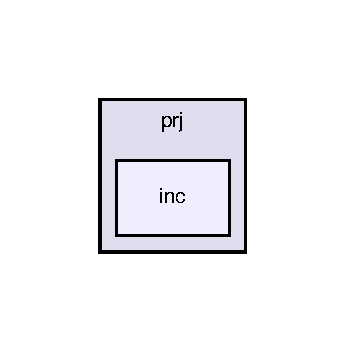
\includegraphics[width=166pt]{dir_acac4094357f78bc086a5e6d3872a7e4_dep}
\end{center}
\end{figure}
\subsection*{\-Pliki}
\begin{DoxyCompactItemize}
\item 
plik \hyperlink{merge_8hpp}{merge.\-hpp}
\begin{DoxyCompactList}\small\item\em \-Plik zawiera definicje funkcji sortowania merge. \end{DoxyCompactList}\item 
plik \hyperlink{quick_8hpp}{quick.\-hpp}
\begin{DoxyCompactList}\small\item\em \-Plik zawiera definicje szablonu sortowania szybkiego. \end{DoxyCompactList}\item 
plik \hyperlink{sort__benchmark_8hpp}{sort\-\_\-benchmark.\-hpp}
\begin{DoxyCompactList}\small\item\em \-Plik zawiera definicje funkcji \-Sort\-\_\-\-Benchmark. \end{DoxyCompactList}\end{DoxyCompactItemize}

\hypertarget{dir_f10a9748acb3706b6d23d4d1158cc82a}{\section{\-Dokumentacja katalogu /home/martyna/pamsi2/lab4.2.1/prj/}
\label{dir_f10a9748acb3706b6d23d4d1158cc82a}\index{\-Dokumentacja katalogu /home/martyna/pamsi2/lab4.\-2.\-1/prj/@{\-Dokumentacja katalogu /home/martyna/pamsi2/lab4.\-2.\-1/prj/}}
}
\-Directory dependency graph for /home/martyna/pamsi2/lab4.2.1/prj/\-:\nopagebreak
\begin{figure}[H]
\begin{center}
\leavevmode
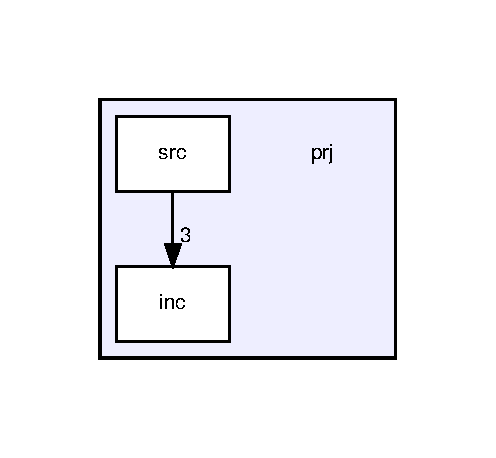
\includegraphics[width=238pt]{dir_f10a9748acb3706b6d23d4d1158cc82a_dep}
\end{center}
\end{figure}
\subsection*{\-Katalogi}
\begin{DoxyCompactItemize}
\item 
katalog \hyperlink{dir_acac4094357f78bc086a5e6d3872a7e4}{inc}
\item 
katalog \hyperlink{dir_f56ce5fa3c89051b057d747031f0cde3}{src}
\end{DoxyCompactItemize}

\hypertarget{dir_f56ce5fa3c89051b057d747031f0cde3}{\section{\-Dokumentacja katalogu /home/martyna/pamsi2/lab4.2.1/prj/src/}
\label{dir_f56ce5fa3c89051b057d747031f0cde3}\index{\-Dokumentacja katalogu /home/martyna/pamsi2/lab4.\-2.\-1/prj/src/@{\-Dokumentacja katalogu /home/martyna/pamsi2/lab4.\-2.\-1/prj/src/}}
}
\-Directory dependency graph for /home/martyna/pamsi2/lab4.2.1/prj/src/\-:\nopagebreak
\begin{figure}[H]
\begin{center}
\leavevmode
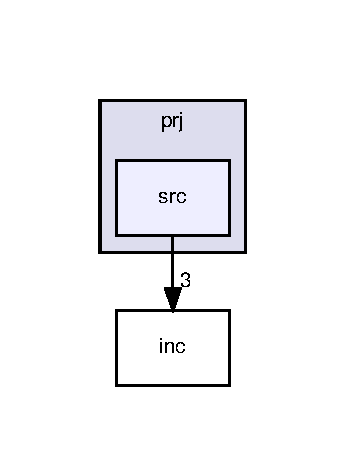
\includegraphics[width=166pt]{dir_f56ce5fa3c89051b057d747031f0cde3_dep}
\end{center}
\end{figure}
\subsection*{\-Pliki}
\begin{DoxyCompactItemize}
\item 
plik \hyperlink{glowny_8cpp}{glowny.\-cpp}
\begin{DoxyCompactList}\small\item\em \-Plik zawiera glowna funkcje programu. \end{DoxyCompactList}\item 
plik \hyperlink{sort__benchmark_8cpp}{sort\-\_\-benchmark.\-cpp}
\begin{DoxyCompactList}\small\item\em \-Benchmark \-Zawiera najważniejsze fukcje programu jak rozmiar tablicy. \-Benchmark sortowanie quick i merge. \end{DoxyCompactList}\end{DoxyCompactItemize}

\chapter{\-Dokumentacja klas}
\hypertarget{class_merge}{\section{\-Dokumentacja klasy \-Merge}
\label{class_merge}\index{\-Merge@{\-Merge}}
}


{\ttfamily \#include $<$merge.\-hpp$>$}

\subsection*{\-Metody publiczne}
\begin{DoxyCompactItemize}
\item 
{\footnotesize template$<$typename T $>$ }\\void \hyperlink{class_merge_a4988abdfdf2abb6b412934bb4c16c80f}{merge} (\-T $\ast$tablica1, int pierwszy, int ostatni)
\item 
{\footnotesize template$<$typename T $>$ }\\void \hyperlink{class_merge_ae0fee8fd920f1abd9c903793a98a6de2}{merge\-\_\-sort} (\-T $\ast$dane, int pierwszy, int ostatni)
\item 
{\footnotesize template$<$typename T $>$ }\\void \hyperlink{class_merge_ae554c22c5112a15381137978188dd3bb}{wypelnij} (\-T $\ast$$\ast$tab, int rozmiar, int procent\-\_\-posortowanych)
\item 
{\footnotesize template$<$typename T $>$ }\\bool \hyperlink{class_merge_a123099309cb142028d6c2d4a0ea66571}{sprawdz\-\_\-porzadek} (\-T $\ast$$\ast$tab, int rozmiar)
\item 
{\footnotesize template$<$typename T $>$ }\\void \hyperlink{class_merge_ab3245c1b49bd123cf24a8168f718775e}{wyswietl} (\-T $\ast$\-Poczatek, \-T $\ast$\-Koniec)
\item 
{\footnotesize template$<$typename T $>$ }\\void \hyperlink{class_merge_a8cbad74164adfdfd8fc922b174885cd1}{wyswietl} (\-T $\ast$$\ast$tab, int rozmiar)
\end{DoxyCompactItemize}


\subsection{\-Dokumentacja funkcji składowych}
\hypertarget{class_merge_a4988abdfdf2abb6b412934bb4c16c80f}{\index{\-Merge@{\-Merge}!merge@{merge}}
\index{merge@{merge}!Merge@{\-Merge}}
\subsubsection[{merge}]{\setlength{\rightskip}{0pt plus 5cm}template$<$typename T $>$ void {\bf \-Merge\-::merge} (
\begin{DoxyParamCaption}
\item[{\-T $\ast$}]{tablica1, }
\item[{int}]{pierwszy, }
\item[{int}]{ostatni}
\end{DoxyParamCaption}
)}}\label{class_merge_a4988abdfdf2abb6b412934bb4c16c80f}
\hypertarget{class_merge_ae0fee8fd920f1abd9c903793a98a6de2}{\index{\-Merge@{\-Merge}!merge\-\_\-sort@{merge\-\_\-sort}}
\index{merge\-\_\-sort@{merge\-\_\-sort}!Merge@{\-Merge}}
\subsubsection[{merge\-\_\-sort}]{\setlength{\rightskip}{0pt plus 5cm}template$<$typename T $>$ void {\bf \-Merge\-::merge\-\_\-sort} (
\begin{DoxyParamCaption}
\item[{\-T $\ast$}]{dane, }
\item[{int}]{pierwszy, }
\item[{int}]{ostatni}
\end{DoxyParamCaption}
)}}\label{class_merge_ae0fee8fd920f1abd9c903793a98a6de2}
\hypertarget{class_merge_a123099309cb142028d6c2d4a0ea66571}{\index{\-Merge@{\-Merge}!sprawdz\-\_\-porzadek@{sprawdz\-\_\-porzadek}}
\index{sprawdz\-\_\-porzadek@{sprawdz\-\_\-porzadek}!Merge@{\-Merge}}
\subsubsection[{sprawdz\-\_\-porzadek}]{\setlength{\rightskip}{0pt plus 5cm}template$<$typename T $>$ bool {\bf \-Merge\-::sprawdz\-\_\-porzadek} (
\begin{DoxyParamCaption}
\item[{\-T $\ast$$\ast$}]{tab, }
\item[{int}]{rozmiar}
\end{DoxyParamCaption}
)}}\label{class_merge_a123099309cb142028d6c2d4a0ea66571}
\hypertarget{class_merge_ae554c22c5112a15381137978188dd3bb}{\index{\-Merge@{\-Merge}!wypelnij@{wypelnij}}
\index{wypelnij@{wypelnij}!Merge@{\-Merge}}
\subsubsection[{wypelnij}]{\setlength{\rightskip}{0pt plus 5cm}template$<$typename T $>$ void {\bf \-Merge\-::wypelnij} (
\begin{DoxyParamCaption}
\item[{\-T $\ast$$\ast$}]{tab, }
\item[{int}]{rozmiar, }
\item[{int}]{procent\-\_\-posortowanych}
\end{DoxyParamCaption}
)}}\label{class_merge_ae554c22c5112a15381137978188dd3bb}
\hypertarget{class_merge_ab3245c1b49bd123cf24a8168f718775e}{\index{\-Merge@{\-Merge}!wyswietl@{wyswietl}}
\index{wyswietl@{wyswietl}!Merge@{\-Merge}}
\subsubsection[{wyswietl}]{\setlength{\rightskip}{0pt plus 5cm}template$<$typename T $>$ void {\bf \-Merge\-::wyswietl} (
\begin{DoxyParamCaption}
\item[{\-T $\ast$}]{\-Poczatek, }
\item[{\-T $\ast$}]{\-Koniec}
\end{DoxyParamCaption}
)}}\label{class_merge_ab3245c1b49bd123cf24a8168f718775e}
\hypertarget{class_merge_a8cbad74164adfdfd8fc922b174885cd1}{\index{\-Merge@{\-Merge}!wyswietl@{wyswietl}}
\index{wyswietl@{wyswietl}!Merge@{\-Merge}}
\subsubsection[{wyswietl}]{\setlength{\rightskip}{0pt plus 5cm}template$<$typename T $>$ void {\bf \-Merge\-::wyswietl} (
\begin{DoxyParamCaption}
\item[{\-T $\ast$$\ast$}]{tab, }
\item[{int}]{rozmiar}
\end{DoxyParamCaption}
)}}\label{class_merge_a8cbad74164adfdfd8fc922b174885cd1}


\-Dokumentacja dla tej klasy została wygenerowana z pliku\-:\begin{DoxyCompactItemize}
\item 
\hyperlink{merge_8hpp}{merge.\-hpp}\end{DoxyCompactItemize}

\hypertarget{class_quick}{\section{\-Dokumentacja klasy \-Quick}
\label{class_quick}\index{\-Quick@{\-Quick}}
}


{\ttfamily \#include $<$quick.\-hpp$>$}

\subsection*{\-Metody publiczne}
\begin{DoxyCompactItemize}
\item 
{\footnotesize template$<$typename T $>$ }\\void \hyperlink{class_quick_a9104bc671992e64990dedf60c0dd6993}{quick\-\_\-sort} (\-T $\ast$\-Poczatek, \-T $\ast$\-Koniec)
\item 
{\footnotesize template$<$typename T $>$ }\\void \hyperlink{class_quick_aad4bc8adc3139667f2edaa1e46993b6e}{wypelnij} (\-T $\ast$$\ast$tab, int rozmiar, int procent\-\_\-posortowanych)
\item 
{\footnotesize template$<$typename T $>$ }\\void \hyperlink{class_quick_a6029457895c0ec57c016c57be5bac0f1}{wypelnij\-\_\-odwrotnie} (\-T $\ast$$\ast$tab, int rozmiar)
\item 
{\footnotesize template$<$typename T $>$ }\\bool \hyperlink{class_quick_abca7e1fcc40e88d337d81aeac1d98184}{sprawdz\-\_\-porzadek} (\-T $\ast$$\ast$tab, int rozmiar)
\item 
{\footnotesize template$<$typename T $>$ }\\void \hyperlink{class_quick_a407bd1912126105f6116393e7676fc05}{wyswietl} (\-T $\ast$\-Poczatek, \-T $\ast$\-Koniec)
\item 
{\footnotesize template$<$typename T $>$ }\\void \hyperlink{class_quick_ab05c6bf9a4fe9d0ed6f83ee02c401ab9}{wyswietl} (\-T $\ast$$\ast$tab, int rozmiar)
\end{DoxyCompactItemize}


\subsection{\-Dokumentacja funkcji składowych}
\hypertarget{class_quick_a9104bc671992e64990dedf60c0dd6993}{\index{\-Quick@{\-Quick}!quick\-\_\-sort@{quick\-\_\-sort}}
\index{quick\-\_\-sort@{quick\-\_\-sort}!Quick@{\-Quick}}
\subsubsection[{quick\-\_\-sort}]{\setlength{\rightskip}{0pt plus 5cm}template$<$typename T $>$ void {\bf \-Quick\-::quick\-\_\-sort} (
\begin{DoxyParamCaption}
\item[{\-T $\ast$}]{\-Poczatek, }
\item[{\-T $\ast$}]{\-Koniec}
\end{DoxyParamCaption}
)}}\label{class_quick_a9104bc671992e64990dedf60c0dd6993}


\-Oto graf wywoływań tej funkcji\-:\nopagebreak
\begin{figure}[H]
\begin{center}
\leavevmode
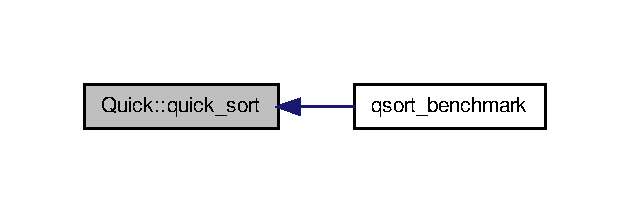
\includegraphics[width=248pt]{class_quick_a9104bc671992e64990dedf60c0dd6993_icgraph}
\end{center}
\end{figure}


\hypertarget{class_quick_abca7e1fcc40e88d337d81aeac1d98184}{\index{\-Quick@{\-Quick}!sprawdz\-\_\-porzadek@{sprawdz\-\_\-porzadek}}
\index{sprawdz\-\_\-porzadek@{sprawdz\-\_\-porzadek}!Quick@{\-Quick}}
\subsubsection[{sprawdz\-\_\-porzadek}]{\setlength{\rightskip}{0pt plus 5cm}template$<$typename T $>$ bool {\bf \-Quick\-::sprawdz\-\_\-porzadek} (
\begin{DoxyParamCaption}
\item[{\-T $\ast$$\ast$}]{tab, }
\item[{int}]{rozmiar}
\end{DoxyParamCaption}
)}}\label{class_quick_abca7e1fcc40e88d337d81aeac1d98184}


\-Oto graf wywoływań tej funkcji\-:\nopagebreak
\begin{figure}[H]
\begin{center}
\leavevmode
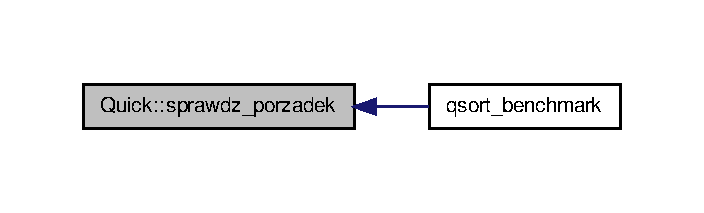
\includegraphics[width=284pt]{class_quick_abca7e1fcc40e88d337d81aeac1d98184_icgraph}
\end{center}
\end{figure}


\hypertarget{class_quick_aad4bc8adc3139667f2edaa1e46993b6e}{\index{\-Quick@{\-Quick}!wypelnij@{wypelnij}}
\index{wypelnij@{wypelnij}!Quick@{\-Quick}}
\subsubsection[{wypelnij}]{\setlength{\rightskip}{0pt plus 5cm}template$<$typename T $>$ void {\bf \-Quick\-::wypelnij} (
\begin{DoxyParamCaption}
\item[{\-T $\ast$$\ast$}]{tab, }
\item[{int}]{rozmiar, }
\item[{int}]{procent\-\_\-posortowanych}
\end{DoxyParamCaption}
)}}\label{class_quick_aad4bc8adc3139667f2edaa1e46993b6e}
\hypertarget{class_quick_a6029457895c0ec57c016c57be5bac0f1}{\index{\-Quick@{\-Quick}!wypelnij\-\_\-odwrotnie@{wypelnij\-\_\-odwrotnie}}
\index{wypelnij\-\_\-odwrotnie@{wypelnij\-\_\-odwrotnie}!Quick@{\-Quick}}
\subsubsection[{wypelnij\-\_\-odwrotnie}]{\setlength{\rightskip}{0pt plus 5cm}template$<$typename T $>$ void {\bf \-Quick\-::wypelnij\-\_\-odwrotnie} (
\begin{DoxyParamCaption}
\item[{\-T $\ast$$\ast$}]{tab, }
\item[{int}]{rozmiar}
\end{DoxyParamCaption}
)}}\label{class_quick_a6029457895c0ec57c016c57be5bac0f1}


\-Oto graf wywoływań tej funkcji\-:\nopagebreak
\begin{figure}[H]
\begin{center}
\leavevmode
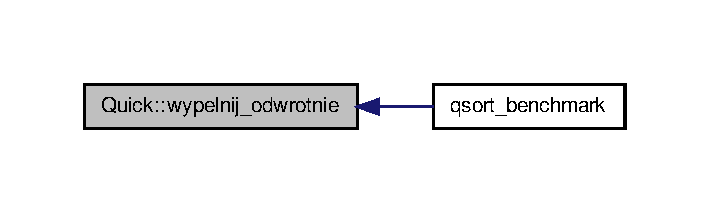
\includegraphics[width=286pt]{class_quick_a6029457895c0ec57c016c57be5bac0f1_icgraph}
\end{center}
\end{figure}


\hypertarget{class_quick_a407bd1912126105f6116393e7676fc05}{\index{\-Quick@{\-Quick}!wyswietl@{wyswietl}}
\index{wyswietl@{wyswietl}!Quick@{\-Quick}}
\subsubsection[{wyswietl}]{\setlength{\rightskip}{0pt plus 5cm}template$<$typename T $>$ void {\bf \-Quick\-::wyswietl} (
\begin{DoxyParamCaption}
\item[{\-T $\ast$}]{\-Poczatek, }
\item[{\-T $\ast$}]{\-Koniec}
\end{DoxyParamCaption}
)}}\label{class_quick_a407bd1912126105f6116393e7676fc05}
\hypertarget{class_quick_ab05c6bf9a4fe9d0ed6f83ee02c401ab9}{\index{\-Quick@{\-Quick}!wyswietl@{wyswietl}}
\index{wyswietl@{wyswietl}!Quick@{\-Quick}}
\subsubsection[{wyswietl}]{\setlength{\rightskip}{0pt plus 5cm}template$<$typename T $>$ void {\bf \-Quick\-::wyswietl} (
\begin{DoxyParamCaption}
\item[{\-T $\ast$$\ast$}]{tab, }
\item[{int}]{rozmiar}
\end{DoxyParamCaption}
)}}\label{class_quick_ab05c6bf9a4fe9d0ed6f83ee02c401ab9}


\-Dokumentacja dla tej klasy została wygenerowana z pliku\-:\begin{DoxyCompactItemize}
\item 
\hyperlink{quick_8hpp}{quick.\-hpp}\end{DoxyCompactItemize}

\chapter{\-Dokumentacja plików}
\hypertarget{glowny_8cpp}{\section{\-Dokumentacja pliku glowny.\-cpp}
\label{glowny_8cpp}\index{glowny.\-cpp@{glowny.\-cpp}}
}
{\ttfamily \#include $<$iostream$>$}\*
{\ttfamily \#include $<$string$>$}\*
{\ttfamily \#include $<$cstdlib$>$}\*
{\ttfamily \#include $<$fstream$>$}\*
{\ttfamily \#include $<$ctime$>$}\*
{\ttfamily \#include \char`\"{}../inc/quick.\-hpp\char`\"{}}\*
{\ttfamily \#include \char`\"{}../inc/tablica.\-hpp\char`\"{}}\*
{\ttfamily \#include \char`\"{}../inc/dzialania.\-hpp\char`\"{}}\*
{\ttfamily \#include \char`\"{}../inc/merge.\-hpp\char`\"{}}\*
\-Wykres zależności załączania dla glowny.\-cpp\-:\nopagebreak
\begin{figure}[H]
\begin{center}
\leavevmode
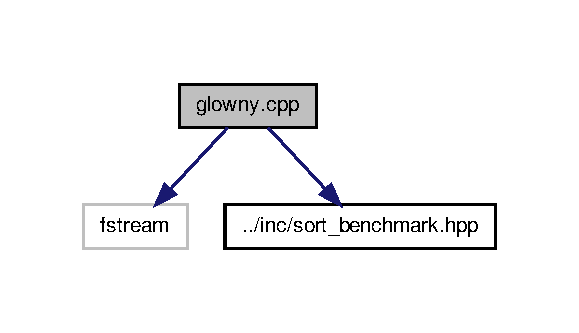
\includegraphics[width=350pt]{glowny_8cpp__incl}
\end{center}
\end{figure}
\subsection*{\-Definicje}
\begin{DoxyCompactItemize}
\item 
\#define \hyperlink{glowny_8cpp_aa50aa866c5823769bb02e986d29a0589}{\-R\-O\-Z\-M\-I\-A\-R}~20
\end{DoxyCompactItemize}
\subsection*{\-Funkcje}
\begin{DoxyCompactItemize}
\item 
int \hyperlink{glowny_8cpp_a3c04138a5bfe5d72780bb7e82a18e627}{main} (int argc, char $\ast$$\ast$argv)
\end{DoxyCompactItemize}


\subsection{\-Dokumentacja definicji}
\hypertarget{glowny_8cpp_aa50aa866c5823769bb02e986d29a0589}{\index{glowny.\-cpp@{glowny.\-cpp}!\-R\-O\-Z\-M\-I\-A\-R@{\-R\-O\-Z\-M\-I\-A\-R}}
\index{\-R\-O\-Z\-M\-I\-A\-R@{\-R\-O\-Z\-M\-I\-A\-R}!glowny.cpp@{glowny.\-cpp}}
\subsubsection[{\-R\-O\-Z\-M\-I\-A\-R}]{\setlength{\rightskip}{0pt plus 5cm}\#define {\bf \-R\-O\-Z\-M\-I\-A\-R}~20}}\label{glowny_8cpp_aa50aa866c5823769bb02e986d29a0589}


\subsection{\-Dokumentacja funkcji}
\hypertarget{glowny_8cpp_a3c04138a5bfe5d72780bb7e82a18e627}{\index{glowny.\-cpp@{glowny.\-cpp}!main@{main}}
\index{main@{main}!glowny.cpp@{glowny.\-cpp}}
\subsubsection[{main}]{\setlength{\rightskip}{0pt plus 5cm}int {\bf main} (
\begin{DoxyParamCaption}
\item[{int}]{argc, }
\item[{char $\ast$$\ast$}]{argv}
\end{DoxyParamCaption}
)}}\label{glowny_8cpp_a3c04138a5bfe5d72780bb7e82a18e627}


\-Glowna funkcja programu. 

\-Wyświetla wynik pomiarowy tablicy. 

\-Oto graf wywołań dla tej funkcji\-:\nopagebreak
\begin{figure}[H]
\begin{center}
\leavevmode
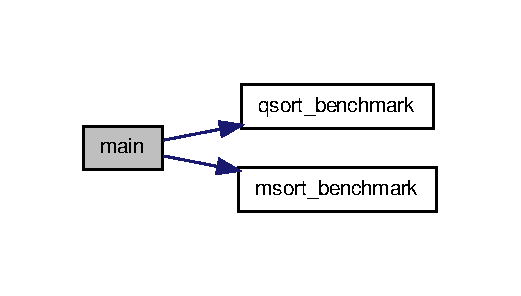
\includegraphics[width=286pt]{glowny_8cpp_a3c04138a5bfe5d72780bb7e82a18e627_cgraph}
\end{center}
\end{figure}



\hypertarget{merge_8hpp}{\section{\-Dokumentacja pliku merge.\-hpp}
\label{merge_8hpp}\index{merge.\-hpp@{merge.\-hpp}}
}


\-Plik zawiera definicje funkcji sortowania merge.  


\-Ten wykres pokazuje, które pliki bezpośrednio lub pośrednio załączają ten plik\-:\nopagebreak
\begin{figure}[H]
\begin{center}
\leavevmode
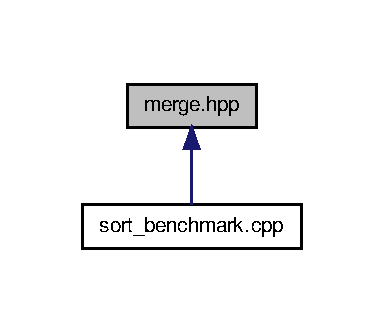
\includegraphics[width=184pt]{merge_8hpp__dep__incl}
\end{center}
\end{figure}
\subsection*{\-Komponenty}
\begin{DoxyCompactItemize}
\item 
class \hyperlink{class_merge}{\-Merge}
\begin{DoxyCompactList}\small\item\em \-Modeluje pojecie \hyperlink{class_merge}{\-Merge}. \-Szablon funkcji sortowania przez scalanie. \end{DoxyCompactList}\end{DoxyCompactItemize}


\subsection{\-Opis szczegółowy}


\-Definicja w pliku \hyperlink{merge_8hpp_source}{merge.\-hpp}.


\hypertarget{quick_8hpp}{\section{\-Dokumentacja pliku quick.\-hpp}
\label{quick_8hpp}\index{quick.\-hpp@{quick.\-hpp}}
}
\-Ten wykres pokazuje, które pliki bezpośrednio lub pośrednio załączają ten plik\-:\nopagebreak
\begin{figure}[H]
\begin{center}
\leavevmode
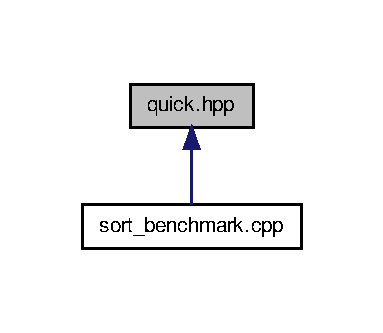
\includegraphics[width=146pt]{quick_8hpp__dep__incl}
\end{center}
\end{figure}
\subsection*{\-Komponenty}
\begin{DoxyCompactItemize}
\item 
class \hyperlink{class_quick}{\-Quick}
\end{DoxyCompactItemize}
\subsection*{\-Funkcje}
\begin{DoxyCompactItemize}
\item 
void \hyperlink{quick_8hpp_acd68a470bbe53460d819b0cea1d7a8e1}{usun\-\_\-tablica} (int $\ast$$\ast$tab)
\end{DoxyCompactItemize}


\subsection{\-Dokumentacja funkcji}
\hypertarget{quick_8hpp_acd68a470bbe53460d819b0cea1d7a8e1}{\index{quick.\-hpp@{quick.\-hpp}!usun\-\_\-tablica@{usun\-\_\-tablica}}
\index{usun\-\_\-tablica@{usun\-\_\-tablica}!quick.hpp@{quick.\-hpp}}
\subsubsection[{usun\-\_\-tablica}]{\setlength{\rightskip}{0pt plus 5cm}void {\bf usun\-\_\-tablica} (
\begin{DoxyParamCaption}
\item[{int $\ast$$\ast$}]{tab}
\end{DoxyParamCaption}
)}}\label{quick_8hpp_acd68a470bbe53460d819b0cea1d7a8e1}


\-Oto graf wywoływań tej funkcji\-:\nopagebreak
\begin{figure}[H]
\begin{center}
\leavevmode
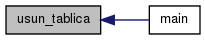
\includegraphics[width=226pt]{quick_8hpp_acd68a470bbe53460d819b0cea1d7a8e1_icgraph}
\end{center}
\end{figure}



\hypertarget{sort__benchmark_8cpp}{\section{\-Dokumentacja pliku sort\-\_\-benchmark.\-cpp}
\label{sort__benchmark_8cpp}\index{sort\-\_\-benchmark.\-cpp@{sort\-\_\-benchmark.\-cpp}}
}


\-Benchmark \-Zawiera najważniejsze fukcje programu jak rozmiar tablicy. \-Benchmark sortowanie quick i merge.  


{\ttfamily \#include $<$iostream$>$}\*
{\ttfamily \#include $<$string$>$}\*
{\ttfamily \#include $<$cstdlib$>$}\*
{\ttfamily \#include $<$fstream$>$}\*
{\ttfamily \#include $<$ctime$>$}\*
{\ttfamily \#include \char`\"{}../inc/quick.\-hpp\char`\"{}}\*
{\ttfamily \#include \char`\"{}../inc/merge.\-hpp\char`\"{}}\*
\-Wykres zależności załączania dla sort\-\_\-benchmark.\-cpp\-:
\nopagebreak
\begin{figure}[H]
\begin{center}
\leavevmode
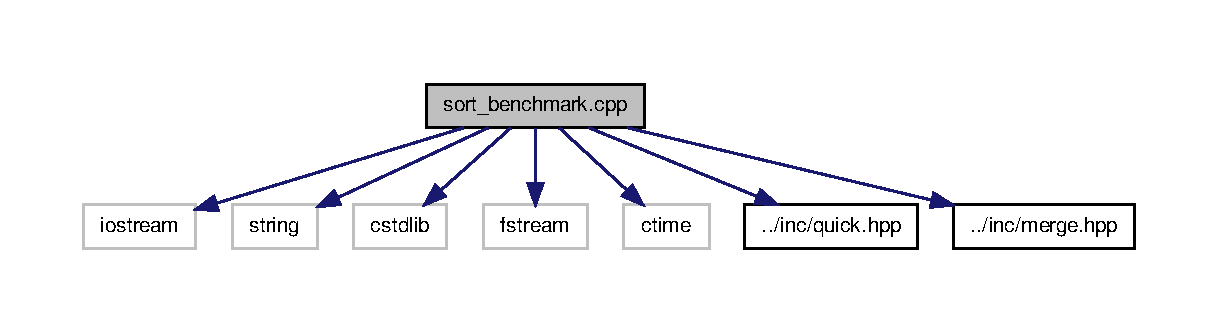
\includegraphics[width=350pt]{sort__benchmark_8cpp__incl}
\end{center}
\end{figure}
\subsection*{\-Funkcje}
\begin{DoxyCompactItemize}
\item 
void \hyperlink{sort__benchmark_8cpp_a0ffe4b68a2d0422a9a851deae952ff3b}{qsort\-\_\-benchmark} (ofstream \&plik)
\item 
void \hyperlink{sort__benchmark_8cpp_a21706a298f523f731440ba123758cff7}{msort\-\_\-benchmark} (ofstream \&plik)
\end{DoxyCompactItemize}
\subsection*{\-Zmienne}
\begin{DoxyCompactItemize}
\item 
int \hyperlink{sort__benchmark_8cpp_a7a94022ad844ead66e9b80459dabdb02}{rozmiar} \mbox{[}$\,$\mbox{]} = \{10000, 50000, 100000, 500000, 1000000\}
\end{DoxyCompactItemize}


\subsection{\-Opis szczegółowy}


\-Definicja w pliku \hyperlink{sort__benchmark_8cpp_source}{sort\-\_\-benchmark.\-cpp}.



\subsection{\-Dokumentacja funkcji}
\hypertarget{sort__benchmark_8cpp_a21706a298f523f731440ba123758cff7}{\index{sort\-\_\-benchmark.\-cpp@{sort\-\_\-benchmark.\-cpp}!msort\-\_\-benchmark@{msort\-\_\-benchmark}}
\index{msort\-\_\-benchmark@{msort\-\_\-benchmark}!sort_benchmark.cpp@{sort\-\_\-benchmark.\-cpp}}
\subsubsection[{msort\-\_\-benchmark}]{\setlength{\rightskip}{0pt plus 5cm}void {\bf msort\-\_\-benchmark} (
\begin{DoxyParamCaption}
\item[{ofstream \&}]{plik}
\end{DoxyParamCaption}
)}}\label{sort__benchmark_8cpp_a21706a298f523f731440ba123758cff7}


\-Definicja w linii 73 pliku sort\-\_\-benchmark.\-cpp.



\-Oto graf wywołań dla tej funkcji\-:\nopagebreak
\begin{figure}[H]
\begin{center}
\leavevmode
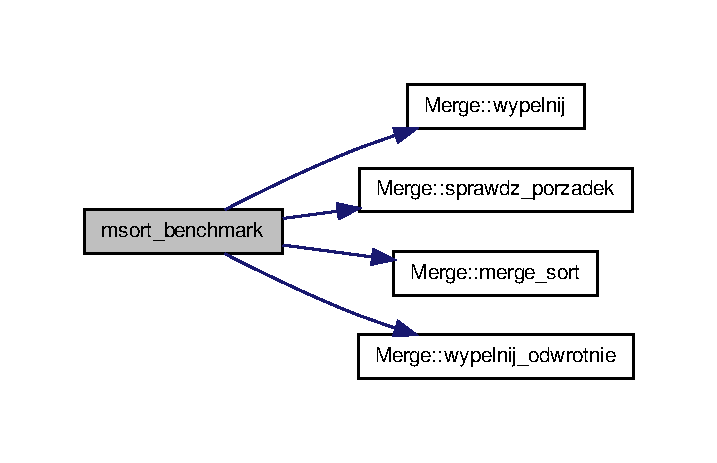
\includegraphics[width=344pt]{sort__benchmark_8cpp_a21706a298f523f731440ba123758cff7_cgraph}
\end{center}
\end{figure}


\hypertarget{sort__benchmark_8cpp_a0ffe4b68a2d0422a9a851deae952ff3b}{\index{sort\-\_\-benchmark.\-cpp@{sort\-\_\-benchmark.\-cpp}!qsort\-\_\-benchmark@{qsort\-\_\-benchmark}}
\index{qsort\-\_\-benchmark@{qsort\-\_\-benchmark}!sort_benchmark.cpp@{sort\-\_\-benchmark.\-cpp}}
\subsubsection[{qsort\-\_\-benchmark}]{\setlength{\rightskip}{0pt plus 5cm}void {\bf qsort\-\_\-benchmark} (
\begin{DoxyParamCaption}
\item[{ofstream \&}]{plik}
\end{DoxyParamCaption}
)}}\label{sort__benchmark_8cpp_a0ffe4b68a2d0422a9a851deae952ff3b}


\-Definicja w linii 21 pliku sort\-\_\-benchmark.\-cpp.



\-Oto graf wywołań dla tej funkcji\-:\nopagebreak
\begin{figure}[H]
\begin{center}
\leavevmode
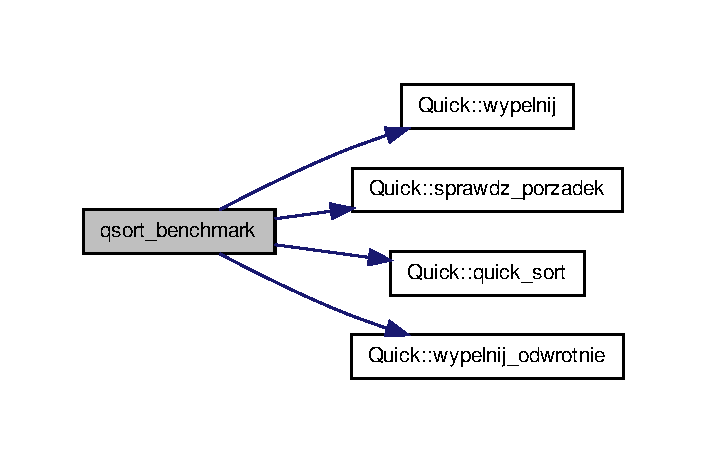
\includegraphics[width=340pt]{sort__benchmark_8cpp_a0ffe4b68a2d0422a9a851deae952ff3b_cgraph}
\end{center}
\end{figure}




\subsection{\-Dokumentacja zmiennych}
\hypertarget{sort__benchmark_8cpp_a7a94022ad844ead66e9b80459dabdb02}{\index{sort\-\_\-benchmark.\-cpp@{sort\-\_\-benchmark.\-cpp}!rozmiar@{rozmiar}}
\index{rozmiar@{rozmiar}!sort_benchmark.cpp@{sort\-\_\-benchmark.\-cpp}}
\subsubsection[{rozmiar}]{\setlength{\rightskip}{0pt plus 5cm}int {\bf rozmiar}\mbox{[}$\,$\mbox{]} = \{10000, 50000, 100000, 500000, 1000000\}}}\label{sort__benchmark_8cpp_a7a94022ad844ead66e9b80459dabdb02}


\-Definicja w linii 18 pliku sort\-\_\-benchmark.\-cpp.


\hypertarget{sort__benchmark_8hpp}{\section{\-Dokumentacja pliku sort\-\_\-benchmark.\-hpp}
\label{sort__benchmark_8hpp}\index{sort\-\_\-benchmark.\-hpp@{sort\-\_\-benchmark.\-hpp}}
}


\-Plik zawiera definicje funkcji \-Sort\-\_\-\-Benchmark.  


\-Ten wykres pokazuje, które pliki bezpośrednio lub pośrednio załączają ten plik\-:\nopagebreak
\begin{figure}[H]
\begin{center}
\leavevmode
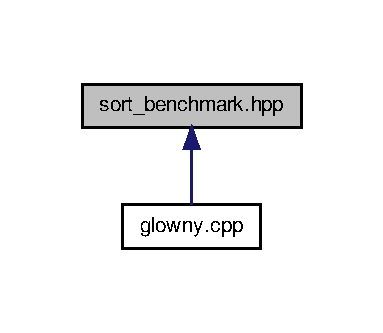
\includegraphics[width=184pt]{sort__benchmark_8hpp__dep__incl}
\end{center}
\end{figure}
\subsection*{\-Funkcje}
\begin{DoxyCompactItemize}
\item 
void \hyperlink{sort__benchmark_8hpp_adab95466b358ff693d939a204772ac3d}{qsort\-\_\-benchmark} (std\-::ofstream \&plik)
\item 
void \hyperlink{sort__benchmark_8hpp_ad82534d3603195ca40af4b0fca16801a}{msort\-\_\-benchmark} (std\-::ofstream \&plik)
\end{DoxyCompactItemize}


\subsection{\-Opis szczegółowy}


\-Definicja w pliku \hyperlink{sort__benchmark_8hpp_source}{sort\-\_\-benchmark.\-hpp}.



\subsection{\-Dokumentacja funkcji}
\hypertarget{sort__benchmark_8hpp_ad82534d3603195ca40af4b0fca16801a}{\index{sort\-\_\-benchmark.\-hpp@{sort\-\_\-benchmark.\-hpp}!msort\-\_\-benchmark@{msort\-\_\-benchmark}}
\index{msort\-\_\-benchmark@{msort\-\_\-benchmark}!sort_benchmark.hpp@{sort\-\_\-benchmark.\-hpp}}
\subsubsection[{msort\-\_\-benchmark}]{\setlength{\rightskip}{0pt plus 5cm}void {\bf msort\-\_\-benchmark} (
\begin{DoxyParamCaption}
\item[{std\-::ofstream \&}]{plik}
\end{DoxyParamCaption}
)}}\label{sort__benchmark_8hpp_ad82534d3603195ca40af4b0fca16801a}


\-Oto graf wywoływań tej funkcji\-:\nopagebreak
\begin{figure}[H]
\begin{center}
\leavevmode
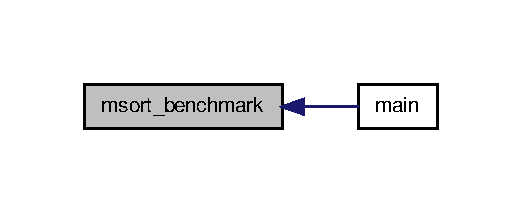
\includegraphics[width=250pt]{sort__benchmark_8hpp_ad82534d3603195ca40af4b0fca16801a_icgraph}
\end{center}
\end{figure}


\hypertarget{sort__benchmark_8hpp_adab95466b358ff693d939a204772ac3d}{\index{sort\-\_\-benchmark.\-hpp@{sort\-\_\-benchmark.\-hpp}!qsort\-\_\-benchmark@{qsort\-\_\-benchmark}}
\index{qsort\-\_\-benchmark@{qsort\-\_\-benchmark}!sort_benchmark.hpp@{sort\-\_\-benchmark.\-hpp}}
\subsubsection[{qsort\-\_\-benchmark}]{\setlength{\rightskip}{0pt plus 5cm}void {\bf qsort\-\_\-benchmark} (
\begin{DoxyParamCaption}
\item[{std\-::ofstream \&}]{plik}
\end{DoxyParamCaption}
)}}\label{sort__benchmark_8hpp_adab95466b358ff693d939a204772ac3d}


\-Oto graf wywoływań tej funkcji\-:\nopagebreak
\begin{figure}[H]
\begin{center}
\leavevmode
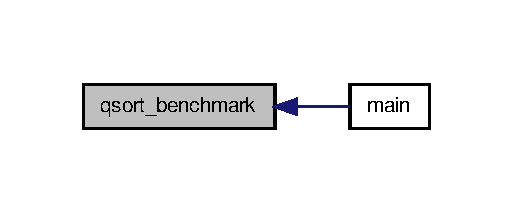
\includegraphics[width=246pt]{sort__benchmark_8hpp_adab95466b358ff693d939a204772ac3d_icgraph}
\end{center}
\end{figure}



\printindex
\end{document}
